\documentclass[12pt]{article}
\usepackage[a4paper, margin=1in]{geometry} 
\usepackage{graphicx} 
\usepackage{hyperref}
\usepackage{float}
\usepackage{multicol}
\usepackage{multirow}
\usepackage{amsmath}
\usepackage[ruled]{algorithm2e}
\usepackage{amssymb}
\usepackage[font=small, labelfont=bf]{caption}

\title{Lecture Notes for \\ INF281 Basics of Bioinformatics Sequence Analysis}
\author{Takaya Saito}
\date{}

\begin{document}

\pagenumbering{arabic}
\setcounter{page}{36}

\makeatletter 
\renewcommand{\thefigure}{\arabic{section}.\arabic{figure}}
\renewcommand{\thetable}{\arabic{section}.\arabic{table}}
\makeatother

%
% PART III
%
\setcounter{part}{2}
\part{}

%
% Database search
%
\setcounter{section}{4}
\setcounter{figure}{0}
\setcounter{table}{0}
\section{Database search}
%\documentclass[12pt]{article}
%\usepackage[a4paper, margin=1in]{geometry} 
%\usepackage{graphicx} 
%\usepackage{hyperref}
%\usepackage{float}
%\usepackage{multicol}
%\usepackage{multirow}
%\usepackage[font=small, labelfont=bf]{caption}
%
%\begin{document}

%
% Biological databases
%
 \subsection{Biological databases}
Biological databases contain biological information, mainly collected from molecular biology experiments, life science literature, and bioinformatics analyses.

%
% Categories of databases
%
\subsubsection*{Categories of databases} 
Annual \href{http://nar.oxfordjournals.org}{Nucleic Acids Research} database issue includes the following database categories.

\begin{itemize}
\item Nucleotide Sequence Databases
\item RNA sequence databases
\item Protein sequence databases
\item Structure Databases
\item Proteomics Resources
\item Human and other Vertebrate Genomes
\item Genomics Databases (non-vertebrate)
\item Plant databases
\item Human Genes and Diseases
\item Metabolic and Signaling Pathways
\item Immunological databases
\item ...
\end{itemize}

%
% GenBank
%
\subsubsection*{GenBank} 
\begin{itemize}
\item A comprehensive database of publicly available nucleotide sequences
\item Produced and maintained by NCBI (National Center for Biotechnology Information, URL: \href{http://www.ncbi.nlm.nih.gov}{http://www.ncbi.nlm.nih.gov})
\end{itemize}

\begin{figure}[H]
  \centering
      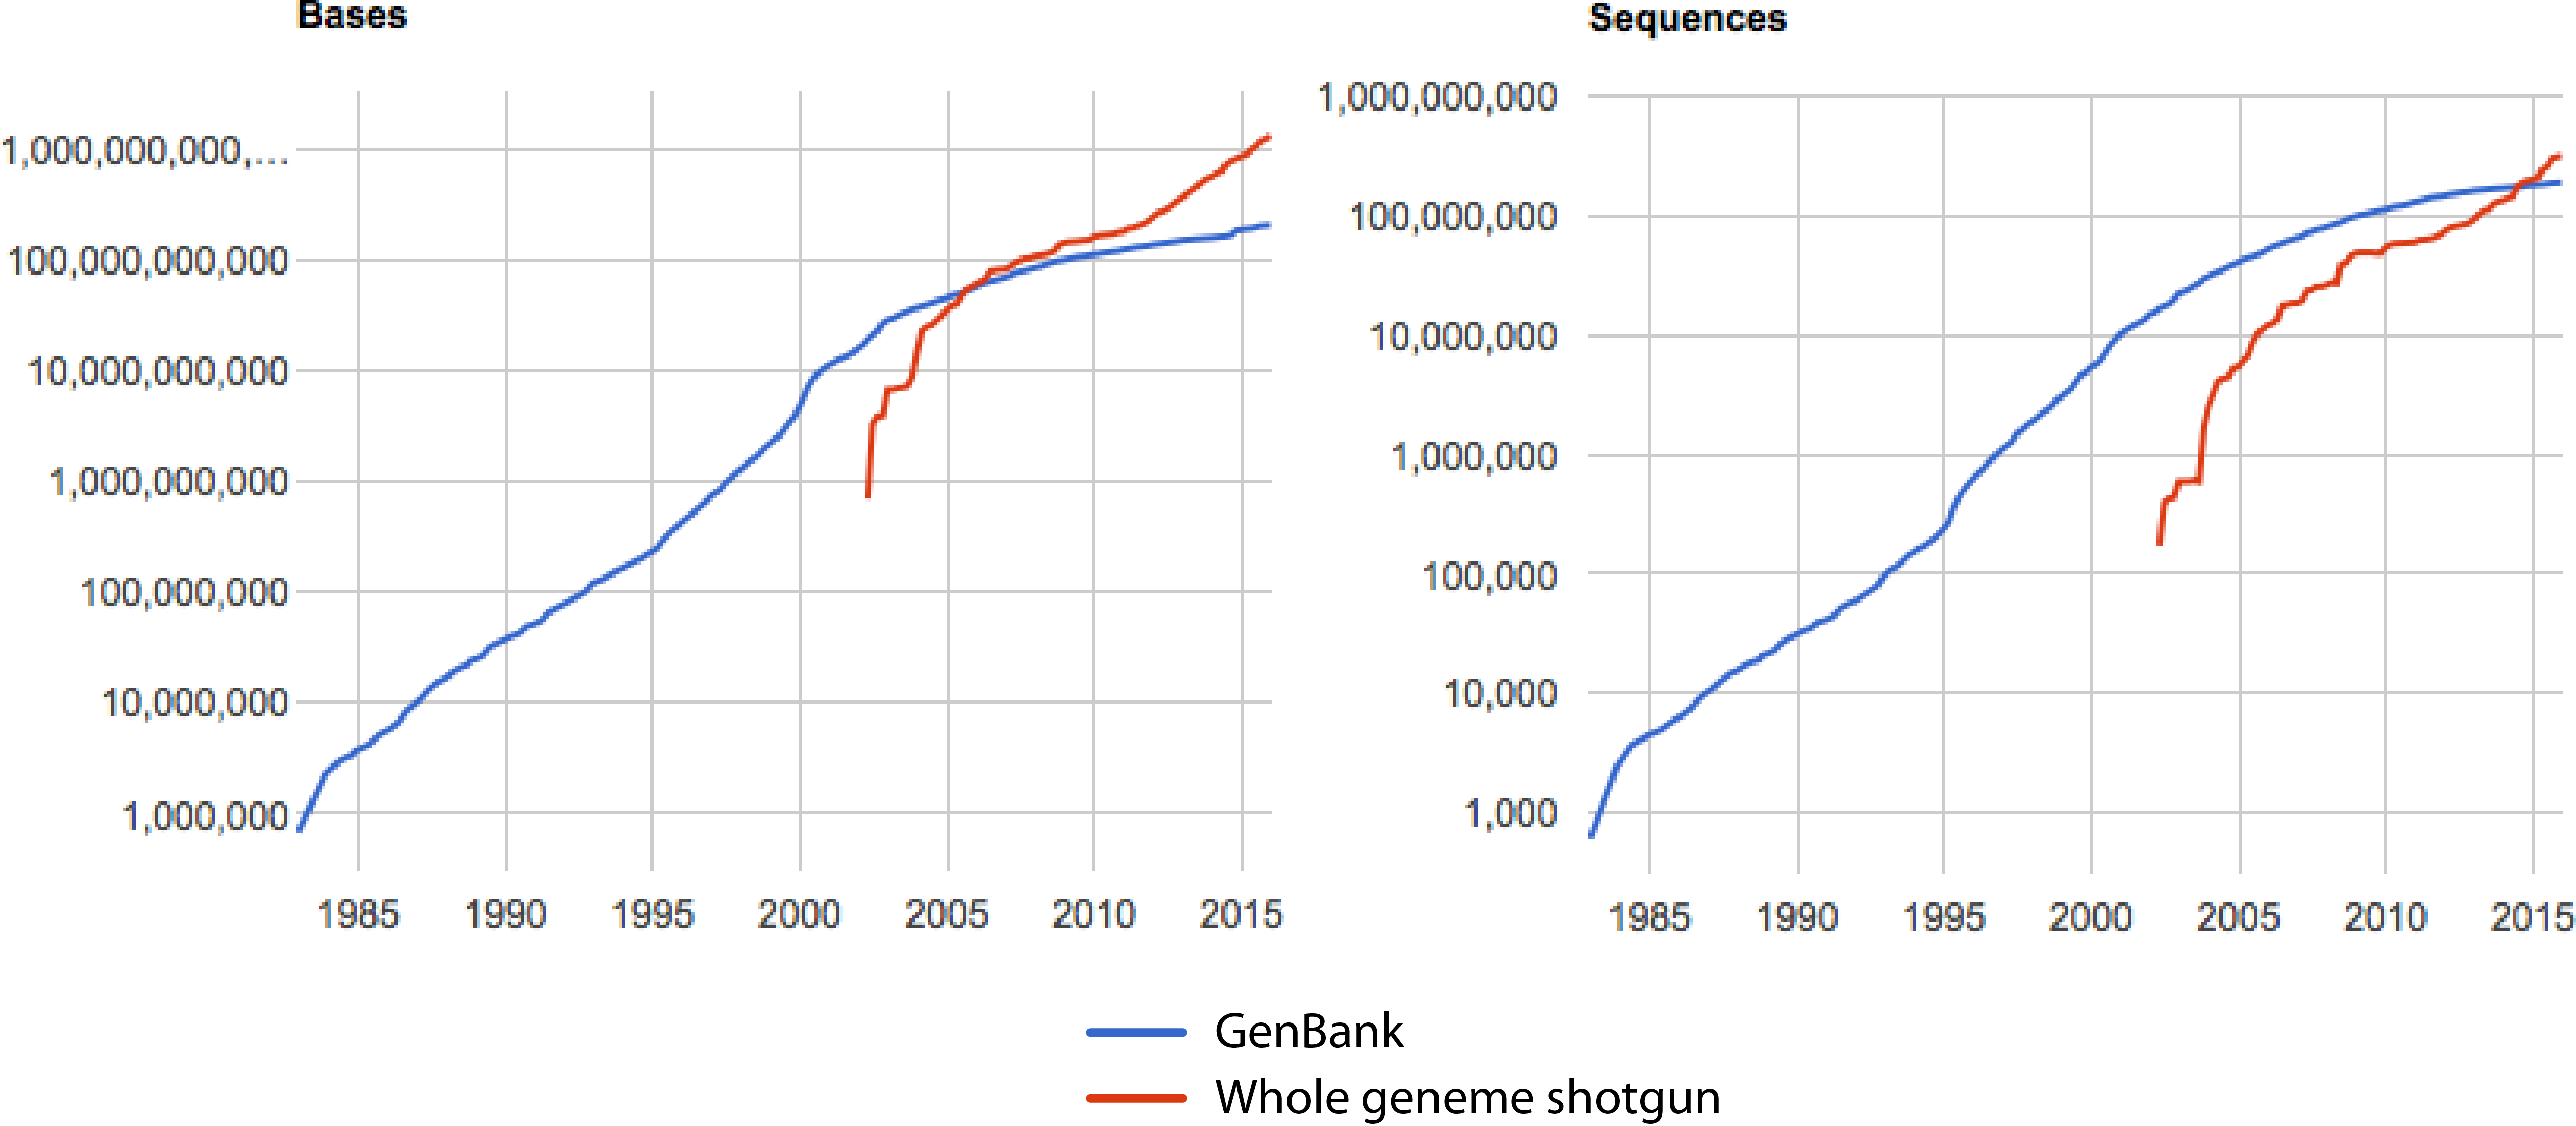
\includegraphics[width=0.6 \textwidth]{fig05/genebank_stat.png}
  \caption{Growth of GenBank and WGS (source: \href{http://www.ncbi.nlm.nih.gov/genbank/statistics}{NCBI})}
\end{figure}

%
% UniProt
%
\subsubsection*{UniProt} 
\begin{itemize}
\item A central repository of protein data from Swiss-Prot, TrEMBL, and PIR-PSD databases
\item Maintained by the UniProt consortium
\end{itemize}

%
% Sequence data 
%
\subsubsection*{Sequence data} 
\begin{itemize}
\item Identifier
\item Sequence
\end{itemize}

\noindent
\textbf{Data format of sequence data} \\
FASTA is the most popular format for sequence data.
\begin{figure}[H]
  \centering
      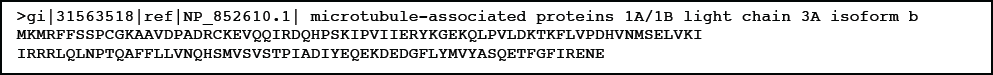
\includegraphics[width=\textwidth]{fig05/fasta.png}
\end{figure}

%
% Annotation data
%
\subsubsection*{Annotation data} 
Sequences databases usually contain annotations in addition to sequences. 

\begin{itemize}
\item Notes and descriptions of important regions and components
\item Meta data
\end{itemize}

\noindent
\textbf{Data format of annotation data} \\
Annotation data can be downloaded in many different formats. GFF is one of the popular file formats for storing genomic features.
\begin{figure}[H]
  \centering
      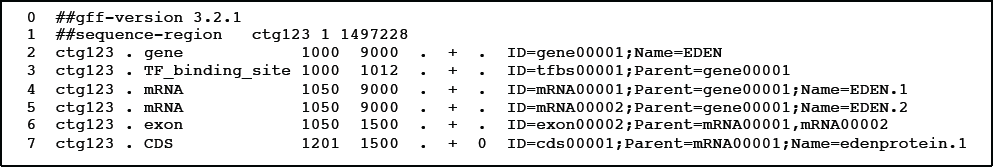
\includegraphics[width=\textwidth]{fig05/gff3.png}
\end{figure}

%
% Tools
%
\subsubsection*{Tools}
Many database tools are available for various purposes.
 
\noindent
\textbf{Search tools for sequence databases}
\begin{itemize}
\item BLAST at NCBI (\href{http://blast.ncbi.nlm.nih.gov/Blast.cgi}{http://blast.ncbi.nlm.nih.gov/Blast.cgi})
\item BLAT/BLAST at Ensembl (\href{http://www.ensembl.org/Multi/Tools/Blast}{http://www.ensembl.org/Multi/Tools/Blast})
\end{itemize}

\noindent
\textbf{Data browsing tools of annotation and sequence data}
\begin{itemize}
\item UCSC Genome Browser (\href{https://genome.ucsc.edu}{https://genome.ucsc.edu})
\item Ensemble Genome Browser (\href{http://www.ensembl.org}{http://www.ensembl.org})
\end{itemize}

\noindent
\textbf{Data download tools for annotation and sequence data}
\begin{itemize}
\item UCSC Table Browser (\href{http://genome.ucsc.edu/cgi-bin/hgTables}{http://genome.ucsc.edu/cgi-bin/hgTables})
\item Ensemble BioMart (\href{http://www.ensembl.org/biomart}{http://www.ensembl.org/biomart})
\end{itemize}

\noindent
\textbf{Tools for protein data}
\begin{itemize}
\item UniProt (\href{https://www.uniprot.org}{https://www.uniprot.org})
\end{itemize}

\bigskip 

%\end{document}

%\documentclass[12pt]{article}
%\usepackage[a4paper, margin=1in]{geometry} 
%\usepackage{graphicx} 
%\usepackage{hyperref}
%\usepackage{float}
%\usepackage{multicol}
%\usepackage{multirow}
%\usepackage[font=small, labelfont=bf]{caption}
%
%\begin{document}

%
% Search in sequence databases
%
\subsection{Search in sequence databases}
Since biological databases contain a large number of sequences, heuristics search methods are usually applied to database search.

%
% Aims of database search
%
\subsubsection*{Aims of searching in sequence databases} 
\begin{itemize}
\item Find homologies 
\item Find segments with important functionality
\end{itemize}

%
% Main procedures of sequence search
%
\subsubsection*{Main procedures of sequence search} 
\begin{itemize}
\item Perform local pairwise alignments
\item Evaluate the alignments statistically
\end{itemize}

%
% Estimated computational time for dynamic programming (DP)
%
\subsubsection*{Estimated computational time for dynamic programming (DP)} 
\begin{table}[h]
\centering
\caption{Estimated computational time of DP for the three cases 1ms, 10ms, and 1sec}
\begin{tabular}{|l|lll|}
\hline
\multirow{2}{*}{\textbf{Time of one alignment}} & \multicolumn{3}{c|}{\textbf{Database size}}                 \\ \cline{2-4} 
                                                & \textbf{1000} & \textbf{1,000,000} & \textbf{1,000,000,000} \\ \hline
\textbf{1 ms}                                   & 1 sec         & 16 min             & 2.6 h                  \\ 
\textbf{10 ms}                                  & 10 sec        & 2.6 h              & 11 days                \\ 
\textbf{1 sec}                                  & 16 min        & 11 days            & 31 years               \\ \hline
\end{tabular}
\end{table}

%
% Heuristic approach
%
\subsubsection*{Heuristic approach} 
\begin{itemize}
\item Need to search billions of entries
\item Tradeoff between accuracy/precision and speed
\item Use n-gram based search
\item BLAST (Basic Local Alignment Search Tool)
\item BLAT (BLAST-like alignment tool)
\end{itemize}

\bigskip 

%\end{document}

%\documentclass[12pt]{article}
%\usepackage[a4paper, margin=1in]{geometry} 
%\usepackage{graphicx} 
%\usepackage{hyperref}
%\usepackage{float}
%\usepackage{multicol}
%\usepackage{multirow}
%\usepackage[font=small, labelfont=bf]{caption}
%
%\begin{document} 

%
% BLAST
%
\subsection{BLAST}
BLAST (Basic Local Alignment Search Tool) is the most popular tool to find homologous sequences in large-scale sequence databases.

%
% Methods
%
\subsubsection*{Methods} 
\begin{itemize}
\item Generate n-grams from query sequence
\item Find n-gram hits in database
\item Expand n-gram hits to HSP
\item Increase HSP scores
\item Introducing gaps
\item Give the expect values (E-values) to HSPs
\end{itemize}

%
% N-gram hits to HSP
%
\subsubsection*{N-gram hits to HSP} 
\begin{itemize}
\item Connect multiple n-gram hits 
\item Increase HSP score
\end{itemize}

\begin{figure}[H]
  \centering
      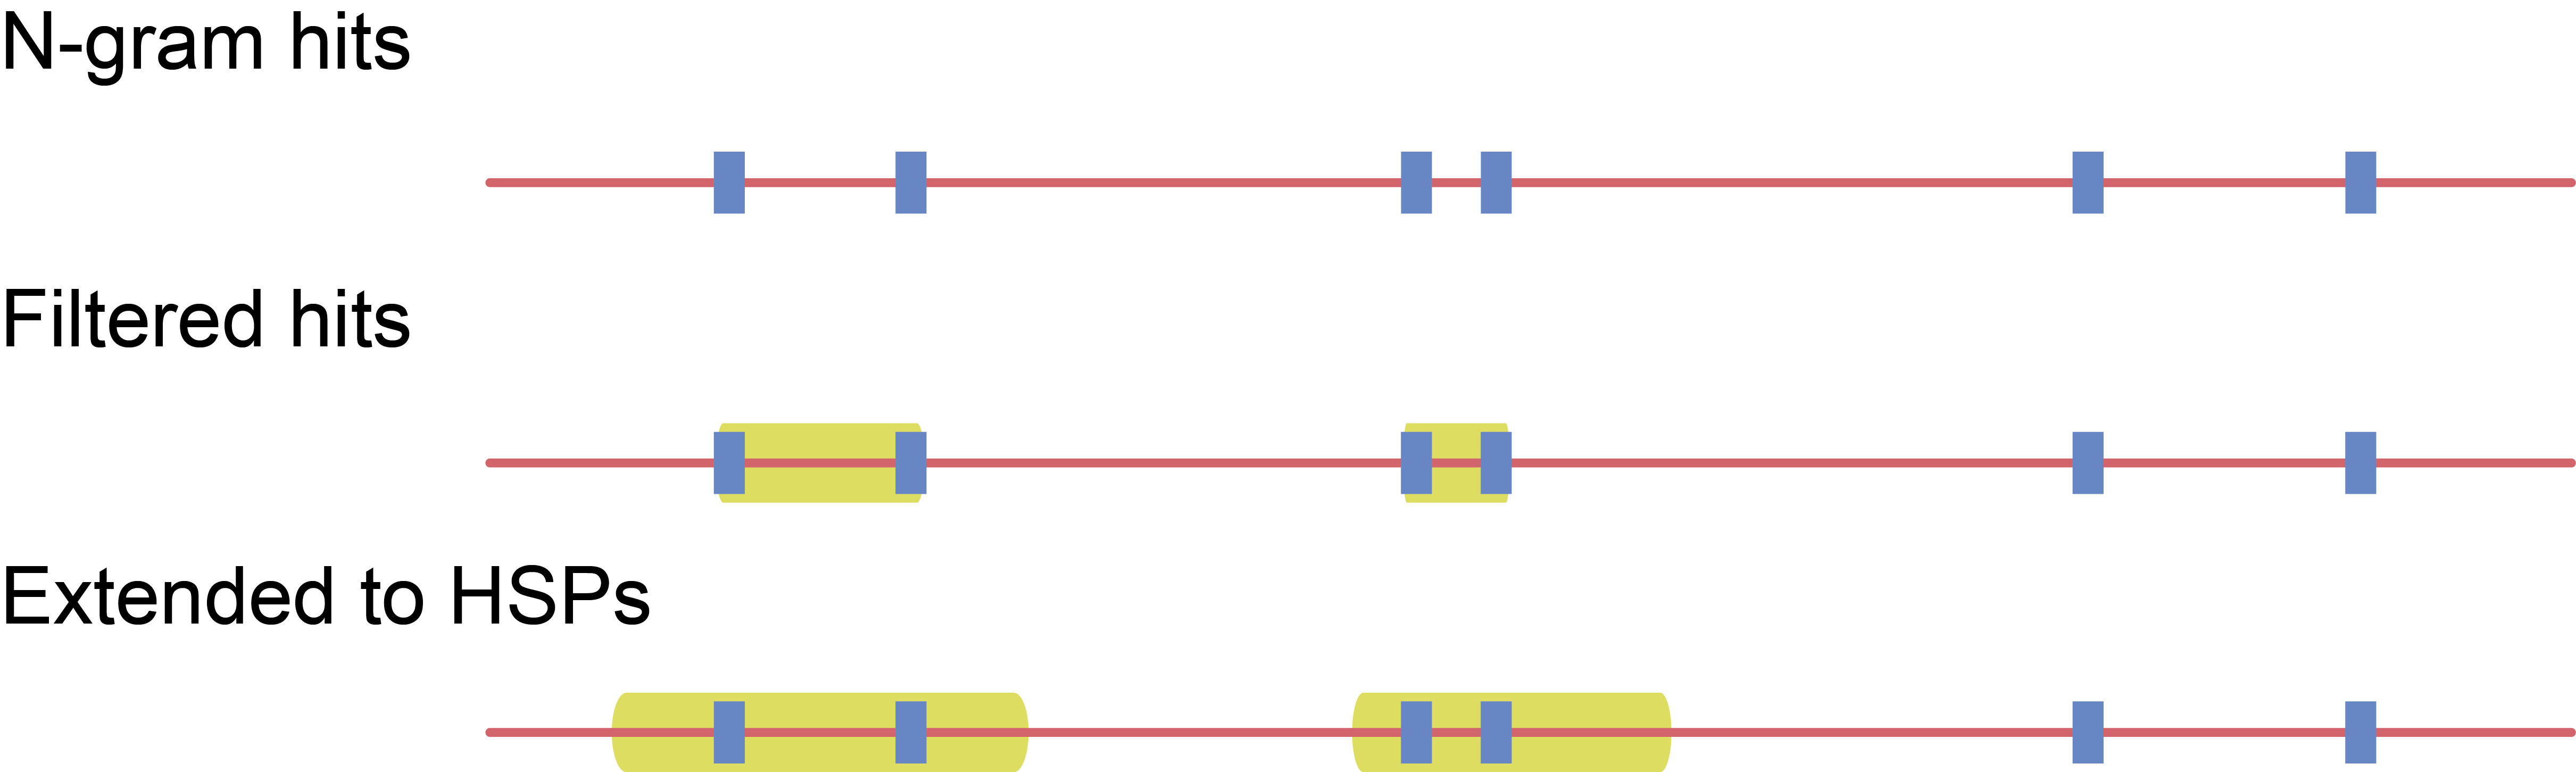
\includegraphics[width=0.75\textwidth]{fig05/extend_hsps.png}
  \caption{N-gram hits to HSPs}
\end{figure}

%
% Increase HSP score
%
\subsubsection*{Increase HSP score} 
BLAST changes the length of HSP by shortening or extending in order to increase the score.

\noindent
\textbf{Example}
\begin{figure}[H]
  \centering
      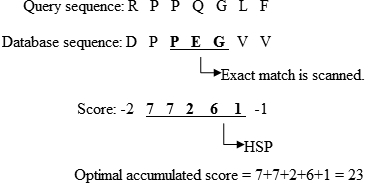
\includegraphics[width=0.45\textwidth]{fig05/extension_process.png}
  \caption{HSP extension process (source: \href{https://commons.wikimedia.org/w/index.php?curid=32912508}{DISP, Wikimedia Commons})}
\end{figure}

%
% Introducing gaps
%
\subsubsection*{Introducing gaps} 
Banded dynamic programming is used to introduce gaps to an HSP.

\begin{figure}[H]
  \centering
      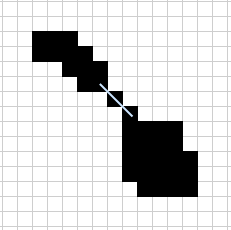
\includegraphics[width=0.25\textwidth]{fig05/banded_dp.png}
  \caption{Banded DP with the starting seed pair}
\end{figure}

%
% E-value
%
\subsubsection*{E-value} 
``The Expect value (E) is a parameter that describes the number of hits one can expect to see by chance when searching a database of a particular size'' \\ \\
-- BLAST Frequently Asked questions (\href{http://blast.ncbi.nlm.nih.gov}{http://blast.ncbi.nlm.nih.gov})

\bigskip 

%\end{document}

%\documentclass[12pt]{article}
%\usepackage[a4paper, margin=1in]{geometry} 
%\usepackage{graphicx} 
%\usepackage{hyperref}
%\usepackage{float}
%\usepackage{multicol}
%\usepackage{multirow}
%\usepackage[font=small, labelfont=bf]{caption}
%
%\begin{document} 

%
% N-gram based search
%
\subsection{N-gram based search}
Using n-grams is a useful method to find segment pairs.

%
% Equivalent or related concepts to n-gram
%
\subsubsection*{Equivalent or related concepts to n-gram} 
\begin{itemize}
\item q-gram
\item n-letter word
\item n-tuple
\item n-mer
\end{itemize}

%
% Create n-grams
%
\subsubsection*{Create n-grams} 
Decomposing a given sequence into n-letter words creates a list of n-grams.

\medskip 

\noindent
\textbf{Example}

\begin{verbatim}
    q: ACGATT 
    
    Word size: 2
        AC, CG, GA, AT, TT
        
    Word size: 3    
        ACG, CGA, GAT, ATT
        
\end{verbatim}

%
% Find segment pairs in database sequences
%
\subsubsection*{Find segment pairs in database sequences} 
N-grams can be used to find segment pairs.

\medskip

\noindent
\textbf{Example}

\begin{verbatim}
    q: ACGATT 
    2-gram: AC, CG, GA, AT, TT
    
    d1: CTAAG
    0 hit

    d2: CGTAT
    2 hits

    d3: ATAGA
    2 hits
\end{verbatim}

\bigskip 

%\end{document}

%\documentclass[12pt]{article}
%\usepackage[a4paper, margin=1in]{geometry} 
%\usepackage{graphicx} 
%\usepackage{hyperref}
%\usepackage{float}
%\usepackage{multicol}
%\usepackage{multirow}
%\usepackage[font=small, labelfont=bf]{caption}
%
%\begin{document} 

%
% Lookup table of matching n-grams
%
\subsection{Lookup table of matching n-grams}
A lookup table can be used for effectively finding n-gram matches.

%
% Terminology
%
\subsubsection*{Terminology} 
\begin{itemize}
\item Indices: positions in q
\item Matching n-grams: Possible matching n-grams by threshold score $T$
\end{itemize}

%
% Example of a creating lookup table
%
\subsubsection*{Example of a creating lookup table} 

\begin{multicols}{2}
\begin{verbatim}
    q: ACGTAC 
    2-gram: AC, CG, GT, TA, AC
    T: 3
\end{verbatim}
\vfill\null
\columnbreak

Score matrix:
\begin{figure}[H]
      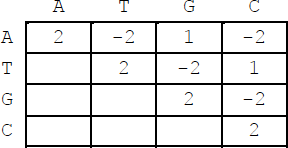
\includegraphics[width=0.25\textwidth]{fig05/score_matrix.png}
\end{figure}

\end{multicols} 

\medskip  

%
% 1. Index of q
%
\subsubsection*{Step 1. Index of q} 
Add indices to all n-grams.

\begin{table}[h]
\small
\begin{tabular}{|l|l|}
\hline
\textbf{Index} & \textbf{N-gram} \\ \hline
1              & AC              \\ \hline
2              & CG              \\ \hline
3              & GT              \\ \hline
4              & TA              \\ \hline
5              & AC              \\ \hline
\end{tabular}
\end{table}


%
% 2. Scores of segment pairs and matching n-grams
%
\subsubsection*{Step 2. Scores of segment pairs and matching n-grams} 

Calculate scores between the first n-gram AC and all its matching n-grams.
\begin{table}[H]
\small
\begin{tabular}{|l|l|l|}
\hline
\textbf{N-gram} & \textbf{Matching n-gram} & \textbf{Score} \\ \hline
AC              & AA                       & $2+(-2)=0$       \\ \hline
AC              & AC                       & $2+2=4$          \\ \hline
AC              & AG                       & $2+(-2)=0$       \\ \hline
AC              & AT                       & $2+1=3$          \\ \hline
AC              & CA                       & $(-2)+(-2)=-4$   \\ \hline
AC              & CC                       & $(-2)+2=0$       \\ \hline
AC              & CG                       & $(-2)+(-2)=-4$   \\ \hline
AC              & CT                       & $(-2)+1=-1$      \\ \hline
AC              & GA                       & $1+(-2)=-1$      \\ \hline
AC              & GC                       & $1+2=3$          \\ \hline
AC              & GG                       & $1+(-2)=-1$      \\ \hline
AC              & GT                       & $1+1=2$          \\ \hline
AC              & TA                       & $(-2)+(-2)=-4$   \\ \hline
AC              & TC                       & $(-2)+2=0$       \\ \hline
AC              & TG                       & $(-2)+(-2)=-4$   \\ \hline
AC              & TT                       & $(-2)+1=-1$      \\ \hline
\end{tabular}
\end{table}

\noindent
Use threshold $T =3$.
\begin{table}[H]
\small
\begin{tabular}{|l|l|l|}
\hline
\textbf{N-gram} & \textbf{Matching n-grams} & \textbf{Scores} \\ \hline
AC              & AC, AT, GC                & 4, 3, 3         \\ \hline
\end{tabular}
\end{table}

\noindent
Repeat the same procedure for all n-grams of q and add their indices.
\begin{table}[H]
\small
\begin{tabular}{|l|l|l|l|}
\hline
\textbf{Index} & \textbf{N-gram} & \textbf{Matching n-grams} & \textbf{Scores} \\ \hline
1              & AC              & AC, AT, GC                & 4, 3, 3         \\ \hline
2              & CG              & CG, TG, CA                & 4, 3, 3         \\ \hline
3              & GT              & GT, AT, GC                & 4, 3, 3         \\ \hline
4              & TA              & TA, CA, TG                & 4, 3, 3         \\ \hline
5              & AC              & AC, GC, AT                & 4, 3, 3         \\ \hline
\end{tabular}
\end{table}

%
% 3. Lookup table of matching n-grams
%
\subsubsection*{Step 3. Lookup table of matching n-grams} 

Transform the table above to create a lookup table of matching n-grams.
\begin{table}[H]
\small
\begin{tabular}{|l|l|l|}
\hline
\textbf{Matching n-gram} & \textbf{Indices of q} & \textbf{Scores of segment pairs} \\ \hline
AC                       & 1, 5                  & 4, 4                             \\ \hline
GC                       & 1, 3, 5               & 3, 3, 3                          \\ \hline
AT                       & 1, 3, 5               & 3, 3, 3                          \\ \hline
CG                       & 2                     & 4                                \\ \hline
TG                       & 2, 4                  & 3, 3                             \\ \hline
CA                       & 2, 4                  & 3, 3                             \\ \hline
GT                       & 3                     & 4                                \\ \hline
TA                       & 4                     & 4                                \\ \hline
\end{tabular}
\end{table}

%
% 4. Search
%
\subsubsection*{Step 4. Search} 

\begin{verbatim}
    d1: AAAGTG 
    
    2 hits
    GT – index: 3, score: 4
    TG – index: (2, 4), score: (3, 3)
\end{verbatim}

%
% Exercise \thesection.1
%
\subsubsection*{Exercise \thesection.1}
Create a lookup table of 2-grams with the indices of q and the scores of segment pairs. Use the threshold $T$ and pre-calculated scores of 2-gram segment pairs.

\begin{verbatim}
    q: CATG
    T: 3
\end{verbatim}

\noindent
The table below shows pre-calculated scores of 2-gram segment pairs.
\begin{table}[H]
\small
\begin{tabular}{|l|l|l|l|}
\hline
\multirow{2}{*}{\textbf{Matching n-gram}} & \multicolumn{3}{c|}{\textbf{N-gram}}    \\ \cline{2-4} 
                                          & \textbf{CA} & \textbf{AT} & \textbf{TG} \\ \hline
AA                                        & 0           & 0           & -1          \\ \hline
AC                                        & -4          & 3           & -4          \\ \hline
AG                                        & -1          & 0           & 0           \\ \hline
AT                                        & -4          & 4           & -4          \\ \hline
CA                                        & 4           & -4          & 2           \\ \hline
CC                                        & 0           & -1          & -1          \\ \hline
CG                                        & 3           & -4          & 3           \\ \hline
CT                                        & 0           & 0           & -1          \\ \hline
GA                                        & 0           & -1          & -1          \\ \hline
GC                                        & -4          & 2           & -4          \\ \hline
GG                                        & -1          & -1          & 0           \\ \hline
GT                                        & 4           & 3           & -4          \\ \hline
TA                                        & 3           & -4          & 3           \\ \hline
TC                                        & -1          & -1          & 0           \\ \hline
TG                                        & 2           & -4          & 4           \\ \hline
TT                                        & -1          & 0           & 0           \\ \hline
\end{tabular}
\end{table}

\bigskip 

%\end{document}

%\documentclass[12pt]{article}
%\usepackage[a4paper, margin=1in]{geometry} 
%\usepackage{graphicx} 
%\usepackage{hyperref}
%\usepackage{float}
%\usepackage{multicol}
%\usepackage{multirow}
%\usepackage[font=small, labelfont=bf]{caption}
%
%\begin{document} 

%
% Finite-state machine with n-grams
%
\subsection{Finite-state machine with n-grams}
Finite-state machine enables efficient database search by expanding the basic n-gram based search.

%
% Number of potential matching n-grams
%
\subsubsection*{Number of potential matching n-grams} 
The number of potential n-grams increases by the alphabet size and the word size.

\medskip 

\noindent
\textbf{DNA} \\
C = \{A, C, G, T\} \\
Word size 2  $\rightarrow$ $4^2$ = 16 \\
Word size 3  $\rightarrow$ $4^3$ = 64 \\
Word size 12  $\rightarrow$ $4^{12}$ = 16,777,216 \\

\noindent
\textbf{Protein} \\
C = \{A, R, N, D, C, Q, E, G, H, I, L, L, M, F, P, S, T, W, Y, V\} \\
Word size 2  $\rightarrow$ $20^2$ = 400 \\
Word size 3  $\rightarrow$ $20^3$ = 8000

%
% Number of potential matching n-grams
%
\subsubsection*{Finite-state machine} 
A finite-state machine can be used to scan database sequences instead of using a lookup table. Finite-state machines are usually faster than lookup tables.

\begin{figure}[H]
  \centering
      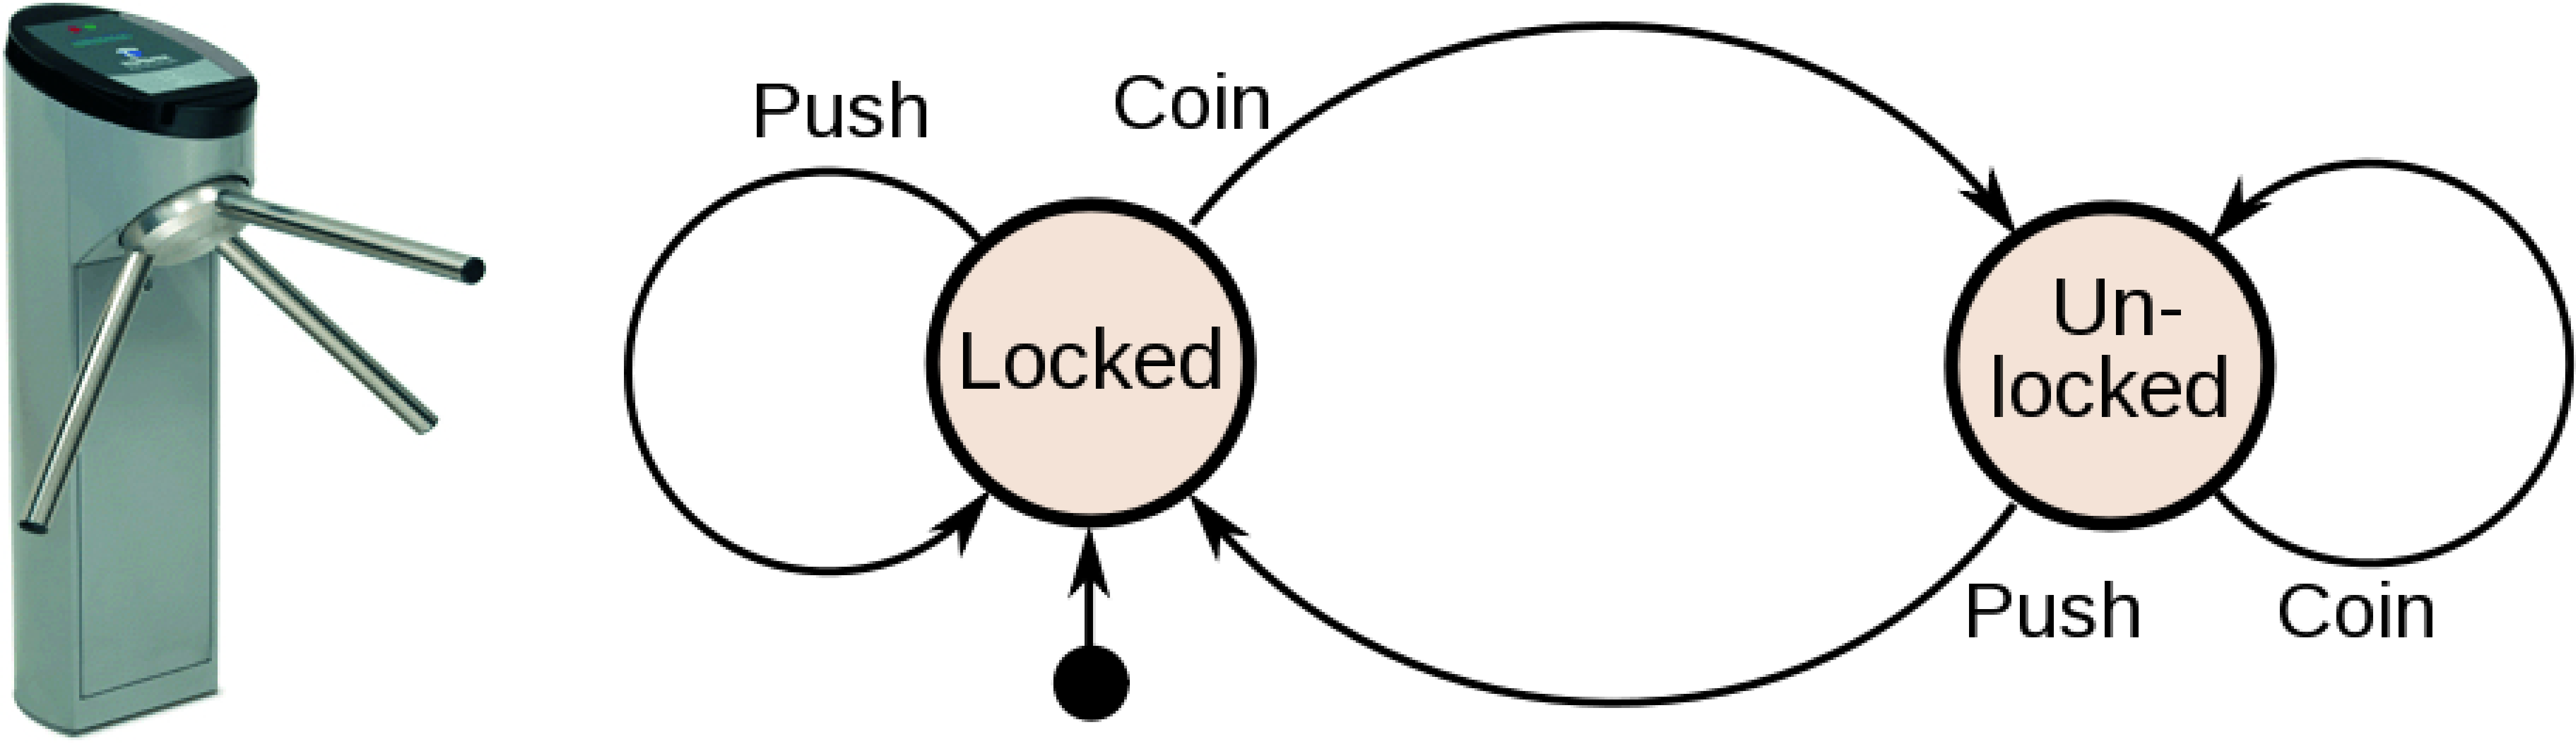
\includegraphics[width=0.6\textwidth]{fig05/fsm_turnstile.png}
  \caption{Finite-state machine for coin-operated turnstile  \newline (sources: \href{https://commons.wikimedia.org/w/index.php?curid=20269475}{Chetvorno} and \href{https://commons.wikimedia.org/w/index.php?curid=8930080}{Sebasgui} via Wikimedia Commons)}
\end{figure}

%
% Example of creating a FSM
%
\subsubsection*{Example of creating a finite-state machine} 

\begin{verbatim}
    q: ACGTAC, Word size: 2, T: 3
\end{verbatim} 

Lookup table
\begin{table}[H]
\small
\begin{tabular}{|l|l|l|}
\hline
\textbf{Matching n-gram} & \textbf{Indices of q} & \textbf{Scores of segment pairs} \\ \hline
AC                       & 1, 5                  & 4, 4                             \\ \hline
GC                       & 1, 3, 5               & 3, 3, 3                          \\ \hline
AT                       & 1, 3, 5               & 3, 3, 3                          \\ \hline
CG                       & 2                     & 4                                \\ \hline
TG                       & 2, 4                  & 3, 3                             \\ \hline
CA                       & 2, 4                  & 3, 3                             \\ \hline
GT                       & 3                     & 4                                \\ \hline
TA                       & 4                     & 4                                \\ \hline
\end{tabular}
\end{table}


\begin{figure}[H]
  \centering
      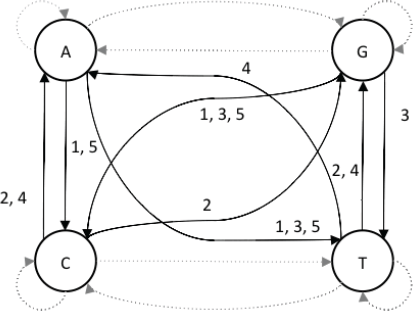
\includegraphics[width=0.4\textwidth]{fig05/fsm_example.png}
  \caption{Finite-state machine to output the indices of 2-grams}
\end{figure}

\begin{verbatim}
    d1: AAAGTG 
    
    2 hits
    GT – index: 3
    TG – index: (2, 4)
\end{verbatim}

%
% Exercise \thesection.2
%
\subsubsection*{Exercise \thesection.2}
Create a finite-state machine and use it to find a segment pair.


\begin{enumerate}
\item Create a finite-state machine for the lookup table for q: ACGTAC. Add both indices and scores to the edges.

\medskip 
Lookup table
\begin{table}[H]
\centering
\small
\begin{tabular}{|l|l|l|}
\hline
\textbf{Matching n-gram} & \textbf{Indices of q} & \textbf{Scores of segment pairs} \\ \hline
AC                       & 1, 5                  & 2, 2                             \\ \hline
CG                       & 2                     & 4                                \\ \hline
GT                       & 3                     & 2                                \\ \hline
TA                       & 4                     & 0                                \\ \hline
\end{tabular}
\end{table}

\item Use the finite-state machine and find a segment pair between q and d: AAAGTG.
\end{enumerate}

\bigskip 

%\end{document}


\end{document}
